\subsection{Módulo de generación de trayectorias}

% B- Módulo de generación de trayectorias
% - Objetivo del módulo	
El objetivo de este módulo es generar trayectorias dentro de la planimetría creada. La modelización de las trayectorias nos permite conseguir una vista preliminar del comportamiento de los algoritmos. Los modelos de movimiento toman importancia en este módulo, ya que de ello dependerá la similitud de los resultados obtenidos con la realidad.
% - Modelización
%       - trayectoria

En Navindoor, las trayectorias están modeladas como una sucesión de puntos dentro de la planimetría. Estos puntos definen los tramos por donde se moverá el activo. Estos se pueden definir con la ayuda de GUI, simplemente haciendo \emph{click} dentro de la planimetría, incluyendo los cambios de planta.

Un vez definida los puntos por donde pasará el activo, con ayuda de modelos de simulación se genera una sucesión de puntos más fina. Esta contiene  coordenadas de los puntos, además del instante de tiempo correspondiente. De esta forma, las velocidades y aceleraciones pueden ser obtenidas mediante diferenciación. Los modelos de generación de la trayectorias en nuestro caso están centrados en la simulación del pie de una persona, por lo que se simula medidas de los sistemas inerciales \emph{foot-mounted}. En concreto se utiliza el modelo propuesto en \cite{Zampella2011}. Además en los casos de cambios de planta se agrega un modelo de velocidad constante.

A partir de la  trayectoria del pie de la persona, se genera la trayectoria del centro de masas. Esta se usará en los casos en el que el sensor esté sobre el tronco de la persona. En la figura \ref{TrajectorySch} se muestra el proceso para la generación de un objeto trayectoria. 

Es importante notar que tanto los modelos de simulación de la trayectoria del pie, como el modelo de generación de la trayectoria del centro de masas, son parámetros opcionales. Es decir, los modelos de simulación son independientes de Navindoor, por lo que nuevos modelos pueden ser implementados creando funciones con la misma interfaz de entrada/salida que las funciones ofrecidas por defecto.

Por último, en la GUI tenemos herramientas para la generación de la trayectoria, desde la opción para crear una sucesión de puntos con \emph{clicks}, pasando por la creación de nuevos modelos, hasta la visualización de la trayectoria generada (figura \ref{fig:animation}).

\begin{figure}[ht!]
    \centering
    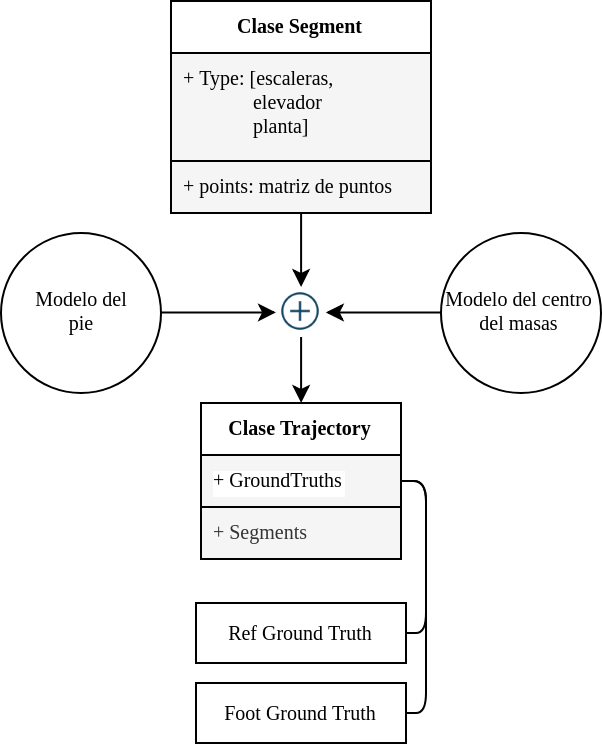
\includegraphics[width=0.75\columnwidth]{img/Design/trajectory.png}
    \caption{Proceso de construcción de una trayectoria.}
    \label{TrajectorySch}
    \footnotesize
    En este esquema se puede ver cómo el constructor de la trayectoria, genera dos objetos \emph{GroundTruths} a partir de segmentos que contienen información extraída de la planimetría. Además, es necesario un modelo que construya la trayectoria del pie de una persona a través de los segmentos y un modelo que sea capaz de crear la trayectoria del centro de masas a partir de la trayectoria del pie. El objeto \emph{Ref GroundTruth} representa la trayectoria del centro de masas, mientras que \emph{Foot GroundTruth} representa la trayectoria del pie de la persona.
\end{figure}



%       - Explicación básica del proceso de generación de trayectorias: 
%       - Selección planta
%       - Clicks con el ratón
%       - Comprobación paredes
%       - Paso a otras plantas
%   - Animación 3D

\begin{figure}
    \centering
    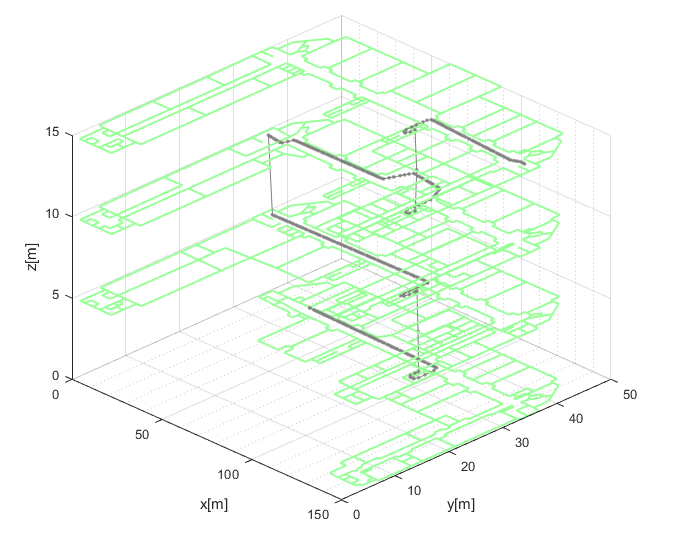
\includegraphics[width=0.8\columnwidth]{img/Design/untitled.png}
    \caption[]{Captura de una animación de una trayectoria}
    \label{fig:animation}
    \footnotesize
    Esta tiene su inicio en la planta cinco y baja usando distintas escaleras y ascensores hasta la primera planta.
\end{figure}
